% EPC flow charts
% Author: Fabian Schuh
\documentclass{minimal}

\usepackage{pgf}
\usepackage{tikz}
\usepackage[utf8]{inputenc}
\usetikzlibrary{arrows,automata}
\usetikzlibrary{positioning}


\tikzset{
    state/.style={
           rectangle,
           rounded corners,
           draw=black, very thick,
           minimum height=2em,
           inner sep=2pt,
           text centered,
           },
}

\begin{document}

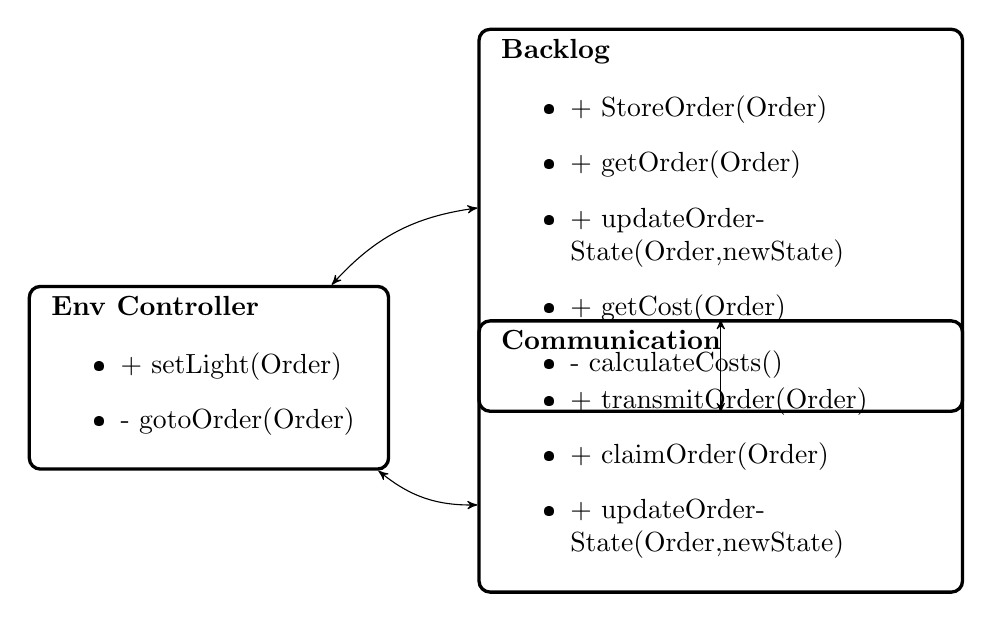
\begin{tikzpicture}[->,>=stealth']

 % Position of Env Controller 
 % Use previously defined 'state' as layout (see above)
 % use tabular for content to get columns/rows
 % parbox to limit width of the listing
 \node[state] (Env Controller) 
 {\begin{tabular}{l}
  \textbf{Env Controller}\\
  \parbox{4cm}{\begin{itemize}
   \item + setLight(Order)
   \item - gotoOrder(Order)
  \end{itemize}
  }
 \end{tabular}};

 \node[state,       % layout (defined above)
  text width=6cm,   % max text width
  yshift=2cm,       % move 2cm in y
  right of=Env Controller,   
  node distance=6.5cm,  
  anchor=center] (Backlog)  % posistion relative to the center of the 'box'
  {\begin{tabular}{l}
  \textbf{Backlog}\\
  \parbox{6cm}{\begin{itemize}
   \item + StoreOrder(Order)
   \item + getOrder(Order)
   \item + updateOrderState(Order,newState)
   \item + getCost(Order)
   \item - calculateCosts()

  \end{itemize}
  }
 \end{tabular}};
 
 % STATE Communication
 \node[state,
  below of=Backlog,
  yshift=-2cm,
  anchor=center,
  text width=6cm] (Communication) 
 {\begin{tabular}{l}
  \textbf{Communication}\\
  \parbox{6cm}{\begin{itemize}
   \item + transmitOrder(Order)
   \item + claimOrder(Order)
   \item + updateOrderState(Order,newState)

  \end{itemize}
  }
 \end{tabular}};

 
 % draw the paths and and print some Text below/above the graph
 \path[<->] (Env Controller)  edge[bend left=20]   (Backlog)
 (Env Controller)        edge[bend right=20]  (Communication)
 %(Communication)     edge[loop below]    node[anchor=north,below]{$SC_n\neq 0$} (Communication)
 (Communication)     edge                 (Backlog);

\end{tikzpicture}
\end{document}